%=====================================================================================
\section{Results}\label{sec:results}
%=====================================================================================
% Sentences marked "% RUN-DEPENDENT" describe learned behaviour (which action each policy
% chose) or the direction of a difference; re-check them whenever the models are retrained.

\subsection{Main Results on Solomon}\label{sec:main}
Table~\ref{tab:compare} reports $T=5{,}000$. The pre-designated seed of \sgalns{} uses
\rcnvSg{} vehicles against \rcnvRw{} for \Rw{} (BKS: \rcnvBks{}), with the lowest gap
(\rgapSg{}\%) and primal integral. In the hierarchical test (Table~\ref{tab:stats}) the
fleet reduction is significant on its own ($\Delta$CNV $=\rstRwdCNV{}$, 95\% CI
$\rstRwciNV{}$, \rstRwpNVt{}) but not after Holm correction over the comparisons of
Table~\ref{tab:stats} (\rstRwpNVholmt{}), and it amounts to 0.06 vehicles per
instance. This is the best of the \rseedN{} training seeds: averaged over all of
them, \sgalns{} uses \rseedCnv{} vehicles. The W/T/L on $f$ (\rcmpRwW{}) is not significant (\rcmpRwPt{}): the
\tTies{} ties are C1/C2 instances solved identically by all methods, and the vehicle
gains come from a few R1, R2 and RC1 instances (Fig.~S3a).
\sgalns{} pulls ahead of all baselines after about 2{,}500 iterations, the end of its
training horizon (Fig.~\ref{fig:analysis}a). Our iteration-level agents are worse than
\sgalns{} and even than \Rw{} (\rcnvIterG{} vehicles), \tIterSlow{}$\times$ slower, and
stall after 1{,}000 iterations. Trained on 100-iteration episodes, both always apply
Worst/Regret-3 (Fig.~\ref{fig:behaviour}a) and return identical solutions. % RUN-DEPENDENT
Even at $T=200$, close to their training horizon, they only match \Rw{}
(\qShortItCnv{} vs.\ \qShortRwCnv{} vehicles), whereas \sgalns{} uses \qShortSgCnv{}
(Table~S16): our iteration-level agents
learned no useful control in either regime, so the comparison does not show that
segment-level decisions are better in general. % RUN-DEPENDENT
Against the two \emph{tuned} baselines,
\sgalns{} is not better in a practically relevant sense: $\Delta$CNV $=\rstRwtdCNV{}$
against tuned \Rw{} (\rstRwtpNVt{}) and $\rstStdCNV{}$ against tuned static
(\rstStpNVt{}), and in both cases TOST shows equivalence within \rdeltaNV{} vehicles
per instance: a difference can be real and still smaller than this margin. At half the
margin, tuned static remains equivalent (\qTostHalfSt{}; all 285 actions: \qTostHalfFull{}),
but tuned \Rw{} does not (\qTostHalfRwt{}). % RUN-DEPENDENT
 No distance
difference is significant. Tuning over all 285 constant
actions instead selects \rfullAct{}, which is equivalent as well ($\Delta$CNV
$=\rstFulldCNV{}$, \rstFullpNVt{}). % RUN-DEPENDENT
In the Friedman--Nemenyi test, \sgalns{}, both tuned baselines and \Rw{} form one
group (Fig.~S4a).

\begin{widefigure}[t]
\centering
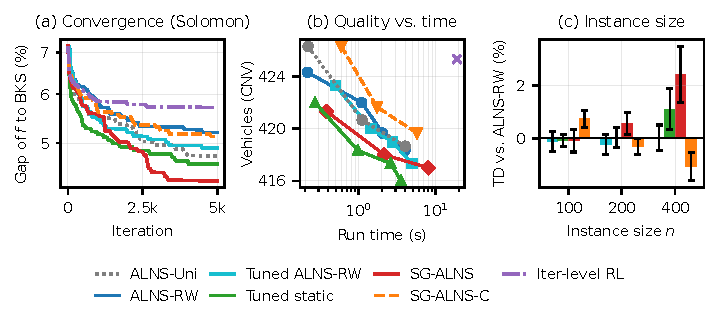
\includegraphics[width=0.76\linewidth]{analysis.pdf}
\caption{(a) Mean gap of the best-so-far $f$ to the BKS during the main phase
(Solomon, 3 seeds; $f$ is dominated by the fleet size). (b) Cumulative vehicles on
Solomon vs.\ mean run time for $T\in\{1,5,10,20\}\cdot10^3$ (3 seeds); points further
down-left are better. (c) Mean relative distance to \Rw{} on instances where both use
the same mean fleet (95\% confidence intervals) for $n=100$ (Solomon), 200 and 400
(Gehring--Homberger).}\label{fig:analysis}
\end{widefigure}

\subsection{Learned Control or Learned Configuration?}\label{sec:collapse}
{\widetables
\begin{table}[t]
\centering
\caption{State-sensitivity probe}\label{tab:probe}
\setlength{\tabcolsep}{3pt}
\begin{adjustbox}{max width=\linewidth}
\begin{tabular}{lccccc}
\toprule
Policy & Natural & Global & Dynamic & No dyn. & Other\\ \midrule
\sgalns{} seed 0 & 0.0 / 0.088 & 0.0 / 0.028 & 0.0 / 0.004 & 0.0 / 0.035 & 0.0 / 0.014\\
seed 1 & 0.0 / 0.129 & 0.0 / 0.028 & 0.0 / 0.011 & 0.0 / 0.151 & 0.0 / 0.055\\
seed 2 & 0.0 / 0.007 & 0.0 / 0.001 & 0.0 / 0.001 & 0.0 / 0.015 & 0.0 / 0.002\\
seed 3 & 31.6 / 0.235 & 57.0 / 0.097 & 6.4 / 0.017 & 23.5 / 0.044 & 21.8 / 0.037\\
seed 4 & 0.0 / 0.008 & 0.0 / 0.002 & 0.0 / 0.002 & 0.0 / 0.014 & 0.0 / 0.007\\
\sgc{} & 0.0 / 0.098 & 0.0 / 0.021 & 0.0 / 0.011 & 0.0 / 0.038 & 0.0 / 0.020\\
neutral prior, seed 0 & 61.8 / 0.211 & 18.1 / 0.083 & 6.8 / 0.018 & 34.6 / 0.120 & 53.3 / 0.079\\
MLP encoder & 0.0 / 0.165 & 0.0 / 0.081 & 0.0 / 0.077 & 0.0 / 0.070 & 0.0 / 0.054\\
w/o expert & 0.0 / 0.086 & 0.0 / 0.024 & 0.0 / 0.014 & 0.0 / 0.070 & 0.0 / 0.036\\
w/o $a^1$ & 92.2 / 0.079 & 7.7 / 0.048 & 4.5 / 0.008 & 37.0 / 0.025 & 18.1 / 0.030\\
$\lambda=1$ & 0.0 / 0.019 & 0.0 / 0.003 & 0.0 / 0.004 & 0.0 / 0.029 & 0.0 / 0.015\\
$\lambda=25$ & 0.0 / 0.027 & 0.0 / 0.006 & 0.0 / 0.001 & 0.0 / 0.013 & 0.0 / 0.016\\
neutral prior, seed 1 & 0.0 / 0.122 & 0.0 / 0.030 & 0.0 / 0.007 & 0.0 / 0.095 & 0.0 / 0.038\\
neutral prior, seed 2 & 0.0 / 0.199 & 0.0 / 0.051 & 0.0 / 0.006 & 0.0 / 0.010 & 0.0 / 0.046\\
seed 0, $5\times$ training & 0.0 / 0.222 & 0.0 / 0.052 & 0.0 / 0.007 & 0.0 / 0.083 & 0.0 / 0.047\\
\bottomrule
\end{tabular}
\end{adjustbox}
\par\vspace{2pt}\parbox{\linewidth}{\footnotesize 12 Solomon instances (two per class, $T=5{,}000$). Each cell: share of queries whose greedy action differs from the action actually taken (\%) / mean total-variation distance between the joint action distributions. Natural: visited states vs.\ the first state of the run; global: progress, temperature, stagnation, gaps, fleet ratio and operator success rates redrawn at random (16 per decision); dynamic: dynamic node features permuted across nodes (4); no dyn.: dynamic node features set to 0; other: graph of another instance (4).}
\end{table}
}
\begin{figure}[!tb]
\centering
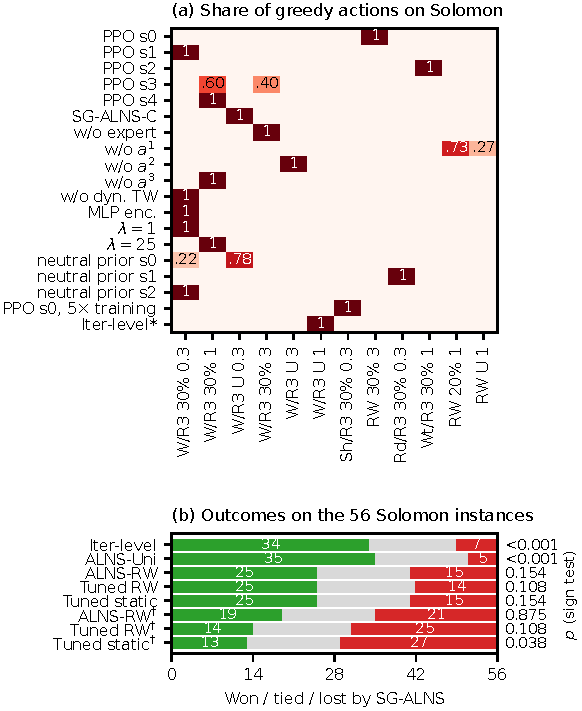
\includegraphics[width=\linewidth]{behaviour.pdf}
\caption{(a) Share of each greedy action over all decisions on Solomon for the
\tNpol{} trained policies (s0, s1, \dots: training seeds; the two iteration-level
agents share a row). Actions are written lead pair, $q$, $m$ with W = Worst, Wt = Wait, Sh = Shaw,
Rd = Random, R3 = Regret-3, U = $\mathcal U[5,30]\%$; ``RW 30\% 3'' is \Rw{} with $q=30\%$ and a
threefold temperature. (b) Instances won, tied and lost by \sgalns{} on $f$, with unadjusted two-sided
sign-test $p$; $^{\dagger}$baselines run with $T=10{,}000$ (equal time).}\label{fig:behaviour}
\end{figure}

\para{Collapse}
In Fig.~\ref{fig:behaviour}a, \tCollapsed{} of the \tNpol{} trained policies choose
\emph{one} action in 100\% of their decisions on Solomon, on every instance. This
includes \sgc{}, which observes $n$ and $T$ yet selects the same action at $n=100$, 200
and 400 and at every budget (Table~S11). Our best policy, seed~0, always selects
\rmainAct{}: it has learned a re-parametrised \Rw{}, not a controller. % RUN-DEPENDENT
Of the three exceptions, training seed~3 and the neutral-prior policy are discussed below;
the third, without $a^1$,
alternates between the default destroy range and
$q=20\%$ (\tNoaSwitch{} switches per run) and uses more vehicles than \sgalns{}
($\Delta$CNV $=\rhNoAdCNV{}$, \rhNoApNVt{}). % RUN-DEPENDENT
Entropy collapses during training (Fig.~S4b), and sampling actions does not change
the result ($\Delta$CNV $=\rhSgsdCNV{}$, \rhSgspNVt{}).
As constancy on test instances does not prove state independence, we probed the
policies (Table~\ref{tab:probe}): for the \qProbeN{} collapsed policies we
probed, \qProbeChg{}\% of about \qProbeQ{} counterfactual queries per policy change the
greedy action, whether the progress, temperature, stagnation and success features are
redrawn at random, the dynamic node features are permuted or zeroed, or the graph is
replaced by that of another instance. The \qProbeReactN{} policies that use several
actions do react (\qProbeReactMin{}--\qProbeReactMax{}\% of queries); two of them, the
variant without $a^1$ and the neutral-prior policy below, perform worse, and the third,
training seed~3, is discussed next. % RUN-DEPENDENT

\para{Training seeds}
If the policy encodes a constant, different training runs may find different ones, and
they do: the \rseedN{} seeds learn \rseedActN{} different actions
(Fig.~\ref{fig:behaviour}a), and \rseedSigN{} of the \rseedN{} use significantly fewer
vehicles than \Rw{} (unadjusted; Table~S3). Seed~3 is the only one that uses its state: it
alternates between \qSthreeActA{} and \qSthreeActB{}, raising the temperature as the
search progresses (the hotter action takes \qSthreeHotFirst{}\% of the decisions in the
first 1{,}000 iterations and \qSthreeHotLast{}\% in the last), much like the best
two-phase schedule below. This learned control, however, is equivalent in fleet size to
tuned static (\qSthreeCnv{} vehicles; $\Delta$CNV $=\qSthreedCnv{}$, \qSthreepNVt{},
TOST). % RUN-DEPENDENT
Likewise, \ifnum\rablWorse=\rablN\relax all \rablN{}\else \rablWorse{} of the \rablN{}\fi{} variants without $a^1$,
$a^2$, $a^3$, dynamic features or message passing use significantly more vehicles than
\sgalns{} (Table~S7), but each is another training run that converged to another
constant; the variants without dynamic features and without message passing even learn
the action of seed~1 and reproduce its results exactly (Fig.~\ref{fig:behaviour}a). % RUN-DEPENDENT
These ablations thus measure seed-to-seed variation, not the value of the encoder or
the features. Conversely, if the controller is a constant, a constant tuned offline
should do as well, and it does: tuned static reaches \rcnvSt{} vehicles at less than
half the run time, and tuned \Rw{} ($q_{\max}=40\%$, $\rho=0.3$) moves \Rw{} from
\rcnvRw{} to \xcnvRwt{} vehicles.

\para{Headroom for control}
A collapse may reflect a weak learner rather than an absence of useful control, so we
searched directly for time-dependent control: all 90 two-phase schedules (one action
per half of the main phase) over the 10 best constant actions, tuned like the
baselines (Table~S6). The best schedule (\vdhA{} $\rightarrow$ \vdhB{}) scores
\vdhDyn{} against \vdhConst{} for the best constant ($p=\vdhP{}$); only \vdhBeat{}
schedules beat it, and one selected on two seeds is worse on the third. On Solomon, the schedule uses as many vehicles as the constant
($\Delta$CNV $=\rhScheddCNV{}$, \rhSchedpNVt{}) but shorter routes ($\Delta$TD
$=\rhScheddTD{}\%$, \rhSchedpTDt{}, \rhSchednTD{} instances). % RUN-DEPENDENT
Time-dependent headroom thus exists; it is small, and a direct search finds it while
none of our policies does. Instance-dependent control has even less room: choosing, with
hindsight, the best of the 15 best constants separately for each Solomon class saves only
\qOrGain{} vehicles over the best single constant (\qOrClassCnv{} vs.\ \qOrSingleCnv{}),
and choosing per class on the generated instances does not help (\qOrSelCnv{}). % RUN-DEPENDENT
PPO hyper-parameters do not appear to cause the collapse: with a constant entropy
coefficient of 0.01 and neutral initial biases, \qEntOne{} of \qEntN{} training seeds
again select a single action, and the third uses \ventN{} actions that differ only in $q$
and has longer routes than \Rw{} ($\Delta$TD $=\rhEntRwdTD{}\%$, \rhEntRwpTDt{}). Nor does
training length: trained five times longer (1{,}500 updates), seed~0 collapses to
\qLongAct{} (\qLongCnv{} vehicles) and ignores counterfactual states (Table~\ref{tab:probe}). Nor does the reward weight: retrained with
$\lambda=1$ and $\lambda=25$, seed~0 again collapses to a single action
(\qLamOneAct{} and \qLamTfAct{}; Table~S15). % RUN-DEPENDENT

\subsection{Equal Time, Budgets and Instance Size}\label{sec:budgets}

\para{Time-matched comparison}
\sgalns{} needs \rtimeSg{}\,s per run against \rtimeRw{}\,s for \Rw{}; features and
inference take only \xpolShareSg{}--\xpolShareCtx{}\% of it (Fig.~S3b), the rest
depends on the selected operators and temperature (tuned static, also with $q=30\%$,
needs \rtimeSt{}\,s). At equal run time, tuned static lies
at or below \sgalns{} except at the shortest budget (Fig.~\ref{fig:analysis}b).
Giving the baselines $T=10{,}000$ roughly equalises run time (\xtmTimeRw{}--\xtmTimeRwt{}\,s,
slightly favouring the tuned baselines). \sgalns{} then still uses fewer vehicles than
\Rw{} ($\Delta$CNV $=\rstRwTmdCNV{}$, \rstRwTmpNVt{}, \rstRwTmpNVholmt{}), but it is
equivalent in fleet size to both tuned baselines, which find shorter routes (tuned \Rw{}: $\Delta$TD
$=\rstRwtTmdTD{}\%$, \rstRwtTmpTDt{}; tuned static: $\rstStTmdTD{}\%$,
\rstStTmpTDt{}) and win more instances than they lose (Fig.~\ref{fig:behaviour}b,
Table~\ref{tab:stats}). % RUN-DEPENDENT

\para{Budgets}
Against tuned static, no fleet difference is significant at any budget, but its sign
flips from $T=1{,}000$ ($\Delta$CNV $=\rbudShortdCNV{}$, \rbudShortpNVt{}), the budget
closest to the training budget of \sgalns{}, to $T=20{,}000$ ($\rbudLongdCNV{}$,
\rbudLongpNVt{}): each constant is best near the budget it was optimised for
(Table~S10). % RUN-DEPENDENT

\para{Instance size}
Fig.~\ref{fig:analysis}c transfers all settings unchanged to $n=200$ and $400$
(Table~S12). The fixed $q=30\%$ learned by \sgalns{} becomes harmful at $n=400$: on
equal-fleet instances its distance is \rbigSgdTD{}\% relative to \Rw{}
(\rbigSgpTDt{}). \sgc{}, trained on $n\le200$, is the best method at $n=400$ (gap
\xhgGapCtxEAA{}\% vs.\ \xhgGapRwEAA{}\% for \Rw{}; $\Delta$TD $=\rbigCtxdTD{}\%$,
\rbigCtxpTDt{}) and matches the gap of tuned \Rw{} at $n=200$ (\xhgGapCtxCAA{}\% vs.\
\xhgGapRwtCAA{}\%), yet it is the weakest learned method on Solomon (\xcnvCtx{}
vehicles). Its advantage at $n=400$ lies in C1, C2, R1 and RC1, not in R2 and RC2 (Table~S17), and
Gehring--Homberger differs from Solomon in more than $n$, so we attribute it to the
training distribution rather than to size alone. As its action is identical at all
sizes, this is not adaptation. % RUN-DEPENDENT

\subsection{Discussion}\label{sec:discussion}
Segment-level RL often finds \emph{good configurations} without hand-tuning, and the
best one we tested when trained on the deployment distribution (\sgc{} at $n=400$).
Its policies, however, are (almost) state-independent, and a direct search finds only
small time-dependent headroom, consistent with~\cite{turkes2021meta}. The differences are also small in practice:
among \sgalns{} and the tuned baselines they stay below \rdeltaNV{} vehicles per
instance, while all methods remain about 13 vehicles above the BKS. This does not
contradict the gains reported in other settings~\cite{kallestad2023,reijnen2024,johnn2024grlos,wang2025ppoalns},
but shows which controls they need before being attributed to adaptation. Why the
policies collapse remains open: neither the entropy schedule, the initial bias, the
reward weight nor five times longer training changes it, leaving the small discrete action space, the discounted
reward and the ease of representing a constant as candidate causes. % RUN-DEPENDENT
\emph{Threats to validity:} our
conclusions concern the VRPTW, our operators and action space, and \rseedN{} training
seeds, not RL control of ALNS in general. Our base ALNS remains about 13 vehicles above
the BKS ($10n$ vehicle-reduction iterations, $T\le20{,}000$), and a stronger base may
change the headroom; the tuned baselines use grids rather than
irace~\cite{lopez2016irace}, and the iteration-level baselines are our re-implementations
rather than the original DR-ALNS or GRLOS code.
